\chapter{Исследовательская часть}

В данном разделе  приведены результаты работы программного обеспечения и проведено измерение и сравнение времени работы  однопоточной и многопоточной реализаций алгоритма обратной трассировки лучей.

\section{Технические характеристики}

Технические характеристики устройства, на котором выполнялось исследование, следующие.

\begin{itemize}
	\item Операционная система Linux Mint 21 \cite{linux}.
	\item Оперативная память: 8 ГБ.
	\item Процессор: Intel(R) Core(TM) i3-10100F CPU @ 3.60 ГГц \cite{intel}.
\end{itemize}

\section{Результаты работы ПО}

На рисунках \ref{img:ex1} и \ref{img:ex2} представлены изображения, полученные с помощью разработанного ПО.

\begin{table}[H]
	\centering
	\begin{tabular}{p{1\linewidth}}
		\centering
		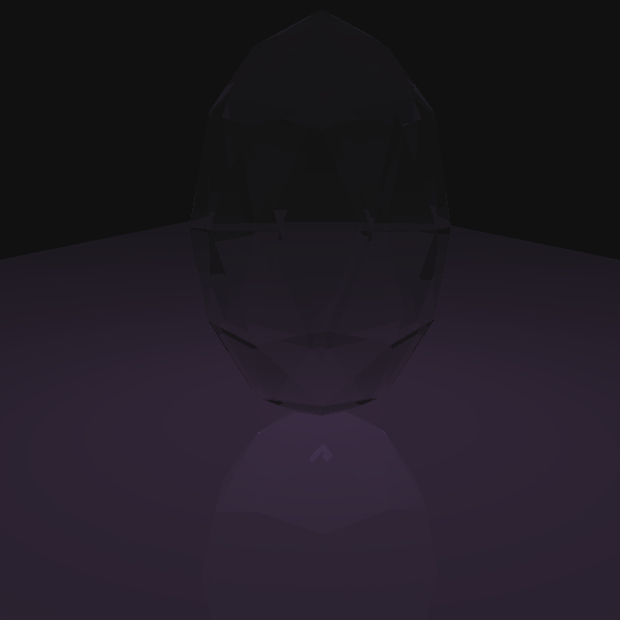
\includegraphics[width=0.64\linewidth]{include/ex1.png}
		\captionof{figure}{Изображение №1, полученное с помощью разработанного ПО}
		\label{img:ex1}
	\end{tabular}
\end{table}

\begin{table}[H]
	\centering
	\begin{tabular}{p{1\linewidth}}
		\centering
		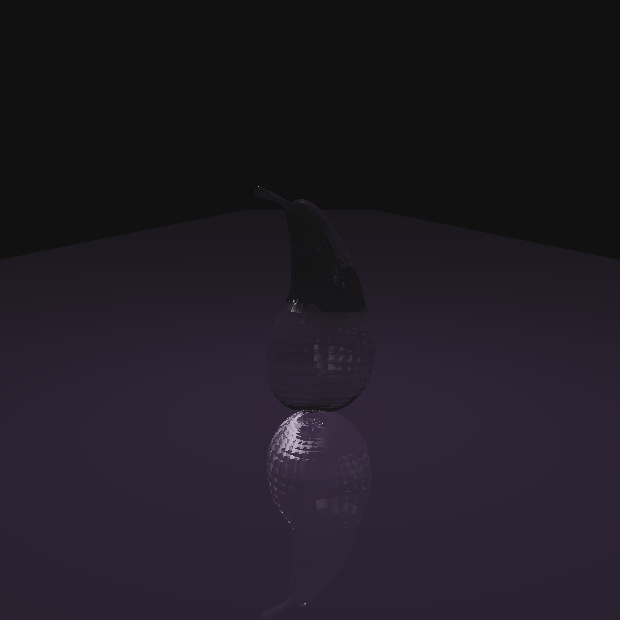
\includegraphics[width=0.64\linewidth]{include/ex2.png}
		\captionof{figure}{Изображение №2, полученное с помощью разработанного ПО}
		\label{img:ex2}
	\end{tabular}
\end{table}

\section{Измерение реального времени выполнения реализаций алгоритма}

Время работы алгоритма обратной трассировки лучей было замерено
с помощью класса \textit{std::chrono::system\_clock} \cite{isocplusplus}, который представляет реальное время. В исследуемых изображениях растр имеет одинаковое количество пикселей в горизонтальном и вертикальном измерениях.

Результаты замеров приведены в таблице \ref{tbl:profilingalgs1}.

\begin{table}[H]
	\begin{center}
		\caption{\label{tbl:profilingalgs1} Таблица времени выполнения алгоритма (мкс.)}
		\begin{tabular}{|c|c|c|c|c|c|c|}
			\hline
			\specialcell{Размер\\изображения\\(в пикселях)} &  \specialcell{Не\\ распарал-\\леленный}    & \multicolumn{5}{|c|}{Количество потоков}\\
			\cline{3-7}
			&   &1&2& 4&8&16\\ 
			
			\hline
			128 & 273311 & 556595 & 339305 & 278957 & 279667 & 292878 \\ \hline
			256 & 2023442 & 3103714 & 1829316 & 1395264 & 1397786 & 1384682 \\ \hline
			352 & 3739262 & 5731390 & 3464986 & 2533300 & 2478940 & 2608794 \\ \hline
			448 & 6302434 & 9693502 & 5783250 & 4178672 & 4100138 & 4188324 \\ \hline
			512 & 9245362 & 13801280 & 8086786 & 5764098 & 5463540 & 6166600 \\ \hline
			640 & 14072760 & 20832840 & 12204240 & 8941954 & 8551252 & 9452858 \\ \hline
			
			
			
		\end{tabular}
	\end{center}
\end{table}

На рисунке \ref{img:plot} приведен графики, отражающий зависимость
времени работы алгоритма обратной трассировки лучей от размера изображения при различном количестве потоков.

\begin{table}[H]
	\centering
	\begin{tabular}{p{1\linewidth}}
		\centering
		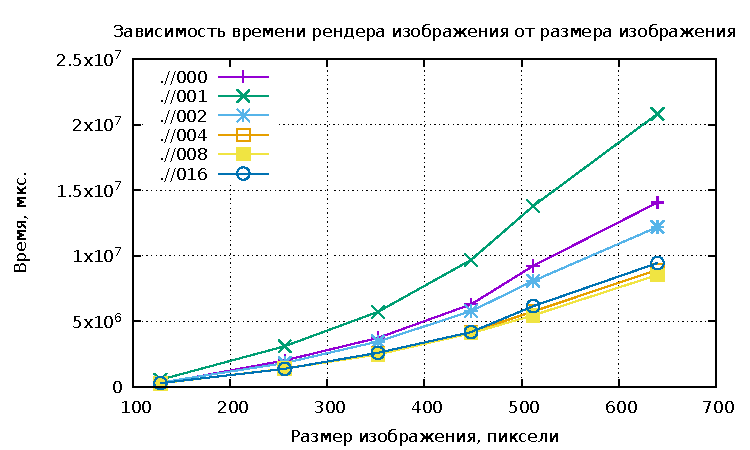
\includegraphics[width=0.81\linewidth]{include/plot.pdf}
		\captionof{figure}{Зависимость
			времени работы алгоритма обратной трассировки лучей от размера изображения при различном количестве потоков}
		\label{img:plot}
	\end{tabular}
\end{table}

\section{Выводы из исследовательской части}

Наилучшее время выполнения параллельный алгоритм показал при 8 потоках, что соответствует количеству логических процессоров компьютера, на котором проводилось измерение. На изображениях размером 640 на 640 пикселей, параллельный алгоритм с 8 потоками работает в $\approx 2,44$ раза быстрее однопоточной реализации. При количестве потоков, большем восьми, время
выполнения увеличивается по сравнению с реализацией с восемью потоками. Таким образом, рекомендуется использовать число потоков, равное числу логических процессоров.
Не распараллеленная реализация работает быстрее однопоточной, поскольку в
однопоточной уходит время на создание потока.